\documentclass[9pt,twocolumn,twoside]{pnas-new}

\usepackage{graphicx}

\templatetype{pnasresearcharticle} 

\title{Crop variety management for climate adaptation supported by citizen science}

\author[a,1*]{Jacob van Etten}
\author[a,b,1]{Kau\^e de Sousa} 
\author[c]{Amílcar Aguilar}
\author[c]{Mirna Barrios}
\author[a]{Allan Coto}
\author[d]{Matteo Dell'Acqua}
\author[e]{Carlo Fadda}
\author[e]{Yosef Gebrehawaryat}
\author[f]{Jeske van de Gevel}
\author[g,h]{Arnab Gupta}
\author[i]{Afewerki Y. Kiros}
\author[a]{Brandon Madriz} 
\author[g]{Prem Mathur}
\author[e,i]{Dejene K. Mengistu}
\author[j]{Leida Mercado}
\author[i]{Jemal Nurhisen Mohammed}
\author[g]{Ambica Paliwal}
\author[d]{Mario Enrico Pè}
\author[a]{Carlos F. Quirós} 
\author[k]{Juan Carlos Rosas}
\author[g,l]{Neeraj Sharma}
\author[m]{S.S. Singh}
\author[n]{Iswhar S. Solanki}
\author[a,o]{Jonathan Steinke}

\affil[a]{Bioversity International, Turrialba, Costa Rica}
\affil[b]{Inland Norway University of Applied Sciences, Department of Agricultural Sciences, Hamar, Norway}
\affil[c]{Tropical Agricultural Research and Higher Education Center (CATIE), Matagalpa, Nicaragua}
\affil[d]{Scuola Superiore Sant'Anna, Institute of Life Sciences, Pisa, Italy}
\affil[e]{Bioversity International, Addis Ababa, Ethiopia}
\affil[f]{Bioversity International, Nairobi, Kenya}
\affil[g]{Bioversity International, Delhi, India}
\affil[h]{Welthungerhilfe, Pathein, Myanmar (current affiliation)}
\affil[i]{Mekelle University, Department of Dryland Crop and Horticultural Sciences, Mekelle, Ethiopia}
\affil[j]{Tropical Agricultural Research and Higher Education Center (CATIE), Turrialba, Costa Rica}
\affil[k]{Zamorano Panamerican Agricultural School, Honduras}
\affil[l]{International Potato Center (CIP), Hanoi, Vietnam (current affiliation)}
\affil[m]{Indian Council for Agricultural Research - Indian Institute of Wheat and Barley Research (ICAR-IIWBR), Karnal (Haryana), India}
\affil[n]{Indian Agricultural Research Institute (IARI), Pusa, Samastipur (Bihar), India}
\affil[o]{Humboldt University of Berlin, Department of Agricultural Economics, Berlin, Germany}

\leadauthor{van Etten} 

\significancestatement{Climate adaptation requires  farmers to adjust their crop varieties over time and use the right varieties to minimize climate risk. Generating variety recommendations for farmers working in marginal, heterogeneous environments requires variety evaluation under farm conditions. On-farm evaluation is difficult to scale with conventional methods. We employed a novel scalable approach to on-farm participatory variety evaluation using crowdsourced citizen science, assigning small experimental tasks to many volunteering farmers. We generated a unique dataset from 12,409 trial plots in Nicaragua, Ethiopia and India, the first participatory variety evaluation dataset of this size and scope. We show the potential of crowdsourced citizen science to generate new insights into variety adaptation, recommend adapted varieties, and help smallholder farmers respond to climate change.}

\authorcontributions{J.v.E., N.S., A.G., P.M., C.F., D.J., J.v.d.G., J.S., Y.G., A.A., L.M., M.B., M.D., M.E.P., I.S.S., S.S.S. and J.C.R. conceived the experiments. N.S., A.G., D.K.M., Y.G., A.A., M.B., J.N.M., A.Y.K., I.S.S and participating farmers conducted the experiments. C.F.Q., B.M. and A.C. developed the digital platform to collect experimental data (www.ClimMob.net). A.P. processed MODIS data. J.v.E. and K.d.S. analyzed the results. J.v.E. wrote the first draft. All authors reviewed the manuscript.}

\authordeclaration{The authors declare no conflict of interest.}

\equalauthors{\textsuperscript{1}J.v.E. and K.d.S. contributed equally to this work.}

\correspondingauthor{\textsuperscript{*}To whom correspondence should be addressed. E-mail: j.vanetten@cgiar.org}

\keywords{Climate adaptation $|$ Genotype x environment interactions $|$ Crop variety evaluation $|$ Citizen science $|$ Crowdsourcing} 

\begin{abstract}
Crop adaptation to climate change requires accelerated crop variety introduction accompanied by recommendations to help farmers match the best variety with their field contexts. Existing approaches to generate these recommendations lack scalability and predictivity in marginal production environments. We tested if crowdsourced citizen science can address this challenge, producing empirical data across geographic space that in aggregate can characterize varietal climatic responses. We present the results of 12,409 farmer-managed experimental plots common bean (\textit{Phaseolus vulgaris} L.) in Nicaragua, durum wheat (\textit{Triticum durum} Desf.) in Ethiopia and bread wheat (\textit{Triticum aestivum} L.) in India. Farmers collaborated as citizen scientists, each ranking the performance of three varieties randomly assigned from a larger set. We show that the approach can register known, specific effects of climate variation on varietal performance. The prediction of variety performance from seasonal climatic variables was generalizable across growing seasons. We show that these analyses can improve variety recommendations in four aspects: reduction of climate bias, incorporation of seasonal climate forecasts, risk analysis, and geographic extrapolation. Variety recommendations derived from the citizen science trials led to important differences with previous recommendations.
\end{abstract}

\dates{This manuscript was compiled on \today}
\doi{\url{www.pnas.org/cgi/doi/10.1073/pnas.XXXXXXXXXX}}

\begin{document}

% Optional adjustment to line up main text (after abstract) of first page with line numbers, when using both lineno and twocolumn options.
% You should only change this length when you've finalised the article contents.
\verticaladjustment{-2pt}

\maketitle
\thispagestyle{firststyle}
\ifthenelse{\boolean{shortarticle}}{\ifthenelse{\boolean{singlecolumn}}{\abscontentformatted}{\abscontent}}{}

% If your first paragraph (i.e. with the \dropcap) contains a list environment (quote, quotation, theorem, definition, enumerate, itemize...), the line after the list may have some extra indentation. If this is the case, add \parshape=0 to the end of the list environment.
\dropcap{C}rop improvement is important to increase agricultural productivity and to contribute to food and nutrition security. The need for new crop varieties is exacerbated by climate change. Farmers need to replace crop varieties with better-adapted ones to match rapidly evolving climate conditions \cite{porter2014chapter, atlin2017rapid,challinor2016current,bellon2011assessing}. Where suitable modern varieties do not exist, suitable farmer varieties are needed instead (‘‘variety’’ is applied to all cultivated materials here) \cite{bellon2011assessing}. The variety replacement challenge is yet to be effectively addressed. One proposed solution is to increase variety supply by accelerating crop breeding, removing older varieties from the seed supply chain and assiduously promoting new varieties for farmers \cite{atlin2017rapid}. Supply-driven variety replacement requires that new varieties are locally adapted and acceptable, but varieties are often recommended without prior geographic analysis to determine recommendation domains, \cite{annicchiarico2002genotype} on the basis of trials that do not adequately represent local production conditions \cite{dawson2008decentralized, atlin2001comparison, ceccarelli2015efficiency}. Therefore, a supply-driven approach may introduce varieties that perform worse than locally-grown varieties. Demand-oriented approaches address this issue, but also fall short of a solution. They involve farmers directly in the selection of crop varieties in on-farm experiments \cite{dawson2008decentralized}. Farmer-participatory selection stimulates local interest in new varieties and produces information on variety performance that is immediately relevant to local climate adaptation. This local focus is a strength as well as a limitation. Scaling is constrained by the resource-intensive nature of current participatory experimental methods and the incompatibility of datasets across different efforts \cite{nelson2016farmer}. The resulting paucity of data is a problem, because variety trials need to capture spatio-temporal environmental variation to characterize climatic responses. 

A solution could come from a more scalable type of participatory research: citizen science using digital ‘‘crowdsourcing’’ approaches \cite{bonney2009citizen,minet2017crowdsourcing,ryan2018role}. This has already shown its potential to engage large numbers of volunteering citizen scientists, who jointly generate sizable datasets that allow geospatial analysis of climate change impact, for example on cross-continental bird migration \cite{cooper2014invisible}. In a similar way, farmer citizen scientists could provide information about crop variety performance, which would feed into a demand-driven, scalable solution to varietal climate adaptation.

To test this idea, we applied a recently developed citizen science approach, \textit{tricot} -- triadic comparisons of technologies \cite{van2011crowdsourcing,van2016first}. In tricot variety evaluation, each farmer plants seeds from a personal test package of three varieties, which are randomly assigned from a larger pool of tested varieties. Farmers' independent on-farm observations are compiled and analyzed centrally. A simple ranking-based feedback format allows even farmers with low literacy skills to contribute their evaluation data through various channels, including mobile telephones \cite{van2016first}. Pilots with the tricot approach have established its potential to produce accurate data \cite{steinke2017accuracy} and to engage motivated farmers as citizen scientists \cite{beza2017prospects}. 

The question we address is if tricot trials can provide robust, actionable information on varietal climate adaptation. We organized tricot trials to obtain a dataset covering 842 plots of common bean in Nicaragua, 1,090 plots of durum wheat in Ethiopia and 10,477 plots of bread wheat in India (Fig. 1). The trials captured environmental variation through broad sampling, both spatially (many fields distributed across the landscape) and temporally (different seasons and planting dates). We linked farmers' observations via their geographic coordinates and planting dates to agroclimatic and soil variables. We modelled the influence of the environmental variables on the probability that varieties outperform the other varieties in the trials. We evaluated whether or not seasonal climate adequately predicts variety performance in the tricot trials. Then, we explored if climatic analysis of tricot trial data improves variety recommendations.

\section*{Characterizing variety performance}
Cross-validation showed that the tricot trials uncovered statistically robust differences in variety performance (Table 1). From a previous pilot study, we expected consistently positive, but low to moderate, pseudo-$R^2$ values \cite{steinke2017accuracy}. In the current study, model fit was comparatively low for bread wheat in India (0.04-0.09), moderate for common bean in Nicaragua (0.15-0.20), and high for durum wheat in Ethiopia (0.39-0.48). The three case studies each provide independent confirmation of the predictive value of the tricot trials. Various factors influenced model fit, including farmers' observation skills and environmental variation. The largest differences were between countries, which were probably due to the different levels of diversity within the sets of varieties. Indian and Nicaraguan farmers evaluated a small, carefully selected group of modern varieties with relatively homogeneous performance. In Ethiopia, farmers tested a diverse set of modern and farmer varieties drawn from a wide area, and evidently found easily observable differences in performance between varieties. 

\begin{figure}[ht!]
\centering
\includegraphics[width=0.5\textwidth]{Fig1_ResearchSites.eps}
\caption{Research sites: \textit{(A)} Overview, \textit{(B)} India, \textit{(C)} Nicaragua, and \textit{(D)} Ethiopia. Farms included in the trials are indicated as dots.}
\label{fig:research_sites}
\end{figure}

\begin{table}[ht]
\centering
\caption{Goodness-of-fit (pseudo-$R^2$) of Plackett-Luce Trees (PLT) determined with 10-fold cross-validation. The model with only climate covariates has the best fit in all cases (indicated in bold).}

\begin{tabular}{@{\extracolsep{8pt}}lrrr@{}}
\hline
PLT model & Nicaragua & Ethiopia & India  \\
\midrule
no covariates & 0.1484 & 0.3947 & 0.0381\\
design & 0.1869 & 0.4709 & 0.0721\\
climate & \textbf{0.1978} & \textbf{0.4870} & \textbf{0.0882}\\
climate + geolocation & 0.1977& 0.4720 & 0.0872\\

\bottomrule
\end{tabular}
\end{table}

For each country, we modeled the environmental influence on variety performance. We were specifically interested in models with covariates derived from seasonal climatic conditions (‘‘climate’’ in Table 1), because these covariates can potentially enhance extrapolation of variety performance predictions across time and space. In all cases, these models had indeed a better fit than the respective model without environmental covariates (‘‘no covariates’’ in Table 1). The next question we addressed was if the models with climatic variables captured the main environmental factors or missed important aspects. Therefore, we compared these models with two other types of models. One type of model includes covariates that represent the experimental design and are known in advance: geolocation, season, planting dates, and soil categories (‘‘design’’ in Table 1). These models reflect how multi-location trials are often analyzed and capture variation in terms of the trial structure but not in terms of the underlying climatic causal factors, hence limiting the potential of extrapolation beyond the trial. In all cases, the models with climatic covariates slightly outperformed the models with trial design covariates. This means that the climatic covariates contain unique and substantial information explaining varietal performance. A second comparison was with models that include the climatic covariates together with additional covariates that represent geographic structure (‘‘climate + geolocation’’ in Table 1). This comparison tested if important local factors are being overlooked that are not covered by the climatic covariates. Adding these geolocational variables did not improve the models, however, and even slightly degraded them. This implies that no large-scale geographical structure remained after accounting for seasonal climate. From this analysis it is clear that the models with climatic covariates captured a large part of the environmental variation in variety performance. Therefore, in subsequent analyses we focused on models with climatic covariates only.

We generated generalizable models that afford extrapolation across seasons of variety performance predictions by selecting those climatic variables that contribute to predictivity across seasons. The variable selection procedure retained one climatic variable in each case (Fig. 2, SI Appendix, Fig. S1). We discuss the results for each case study. 

For Nicaragua, Fig. 2 shows the Plackett-Luce Tree with the retained variable of the generalizable model for common bean. We found that bean variety performance changed when the maximum night temperature exceeded 18.7$^{\circ}$C. 
This finding corresponds to the threshold temperature for heat stress reported in the literature of 20$^{\circ}$C at night \cite{rainey2005inheritance}. Our estimate is slightly lower than the reported threshold, but refers to land-surface temperature rather than air temperature. Three bean varieties, INTA Fuerte Sequía, BRT 103-182, and INTA Centro Sur performed better than the local variety above the heat stress threshold. These three varieties are known to be heat tolerant. Contrary to our expectations, another heat-tolerant variety, SJC 730-79, did not show a performance advantage above 18.7$^{\circ}$C. Above higher heat stress thresholds, however, this variety did outperform heat-sensitive varieties. The group of local varieties has a small quasi-standard error, despite the diverse nature of this group, which contains all varieties farmers currently grow. This gives a reference on farmers' overall appreciation of the tested varieties in comparison to their own varieties. The local varieties were outperformed under heat stress, but not under cool conditions. 

For durum wheat in Ethiopia, varietal differences in performance were related to the lowest night temperature during the vegetative period (SI Appendix, Fig. S2). Performance patterns changed when at least one 8-day period had average night temperatures under 8.4$^{\circ}$C. This temperature corresponds to the threshold temperatures for vernalization and cold acclimation induction \cite{fowler2008cold}. Under warm conditions, vernalization-requiring varieties will delay flowering. Under cold conditions, cold-sensitive varieties will reduce their yield due to chilling or frost damage. Most of the varieties tested in Ethiopia were farmer varieties and likely adapted to their original environments, which may have led to differences in adaptiveness between varieties. To test the effect of local adaptation, we compared cold-adapted with cold-sensitive farmer varieties, as detected by the tricot trials (Methods). Cold-adapted varieties came from higher elevations (2483 $\pm$ 113 masl) than cold-sensitive ones (2101 $\pm$ 485 masl), a significant difference ($t(594)=16.1$, $p<2.2 \cdot 10^{-16}$). Our results indicate that cold tolerance is a main geographic adaptation factor for durum wheat in the Ethiopian highlands.

\begin{figure}[ht!]
\centering
\includegraphics[width=0.48\textwidth]{Fig2_PLTrees.eps}
\caption{Plackett-Luce Tree of tricot trial data and associated climatic data for common bean in Nicaragua. The horizontal axis of each panel is the probability of winning of varieties. Error bars show quasi-standard errors. The grey vertical lines indicate the average probability of winning (1 / number of varieties). In this case, the model selected maxNT, the maximum night temperature ($^{\circ}$C) during the vegetative and flowering periods, as the covariate. Equivalent figures for the trials in Ethiopia and India are shown in SI Appendix, Fig. S2 and Fig. S3}
\label{fig:trees}
\end{figure}

For bread wheat in India, varietal performance patterns changed with the diurnal temperature range (DTR) during the vegetative period, which is the difference between minimum and maximum daily temperature (SI Appendix, Fig. S3). Splits occurred at DTR values of 14.5$^{\circ}$C and 15.7$^{\circ}$C. Between these two values, the varieties showed very similar performance. Many varieties that performed above average under high DTR performed below average under low DTR and vice versa. Some varieties performed well under both high and low DTR, especially HD 2967. Our interpretation is that low and high ranges of DTR are related to different sets of stresses, while the middle range has relatively low stress. DTR has an impact on crop yield through several mechanisms: high DTR is associated with increased heat or cold stress and low DTR is associated with high cloud coverage, low solar radiation and high rainfall. Consistent with our results, a study has shown that DTR explains a substantial share of wheat yield variation in India \cite{rao2015spatial}. This same study found that DTR has a negative correlation with wheat yields in some areas, and a positive correlation in other areas, in line with high and low DTR having an association with different types of crop stress.

\section*{Improving variety recommendations} 

We examined four ways in which climatic analysis afforded by tricot trials can improve variety recommendations. A first potential improvement is that climatic analysis corrects the climatic sampling bias, a bias that occurs when trials are performed under unrepresentative seasonal climate conditions, thereby degrading variety recommendations. To assess the importance of climatic sampling bias, we followed the cross-validation procedure used to generate the generalizable models, but did not use the seasonal climate data for predictions. Instead, we predicted variety performance for a representative 15-year base period of seasonal climate data and averaged the results (Table 2, ‘‘average season’’). The averaged prediction had slightly higher pseudo-$R^2$ values than the ‘‘no covariates’’ model in all cases. This analysis shows that even when climatic sampling bias is low, correction can help to further improve predictions. 

\begin{table}[ht]
\centering
\caption{Goodness-of-fit (pseudo-$R^2$) of generalizable Plackett-Luce Tree models. Model ‘‘average season’’ corrects for climatic sampling bias by averaging predictions over a base period of seasonal climate data. Model ‘‘perfect forecast’’ uses observed climatic covariates in the predicted seasons. Values represent cross-validated pseudo-R\textsuperscript{2} values averaged across blocks, weighted with the square root of the sample size of each block.}

\begin{tabular}{@{\extracolsep{8pt}}lrrrr@{}}
\hline

Model           & Nicaragua  & Ethiopia & India \\
\midrule
no covariates  & 0.1533 & 0.4280    & 0.0611\\
average season   & 0.1536 & 0.4290    & 0.0694\\
perfect forecast & 0.1749 & 0.4442    & 0.1065\\

\bottomrule
\end{tabular}

\end{table}

\begin{table}[ht]
\centering
\caption{Expected probability of winning (average of all farms over the base period) and worst regret measures of a subset of the varieties. The results show how different criteria of variety selection can lead to different recommendations (best value according to each criterion indicated in bold). Using the probability of winning as a criterion maximizes the average performance, but ignores risk. Minimizing worst regret (the loss under the worst possible outcome) is a criterion that takes a conservative approach to risk.}

\begin{tabular}{@{\extracolsep{8pt}}lrrrr@{}}
\hline

Case study &  Variety & Probability  & Worst   \\
 &   & of winning &  regret \\
\midrule
Common bean &  	Local variety & 	\textbf{0.130} & 	0.023 \\
(Nicaragua) & 	INTA Fuerte Sequía & 0.125 & 			\textbf{0.021} \\
 			&  	INTA Centro Sur & 	0.098 &				0.057 \\
 			&  	BRT 103-182 & 		0.092 & 			0.068 \\
 			&  	INTA Rojo & 		0.088 & 			0.082 \\
 			&  	INTA Matagalpa & 	0.087 & 			0.057 \\
 \midrule
Durum wheat & 	208279 & 	\textbf{0.059} & 	0.062 \\ 
(Ethiopia) & 	Hitosa & 	0.049 & 			\textbf{0.035} \\ 
 		& 		208304 & 	0.041 & 			0.048 \\ 
 		& 		8034 & 		0.030 & 			0.053 \\ 
 		& 		Ude & 		0.025 & 			0.063 \\ 
        & 		222360 & 		0.023 & 			0.061 \\ 
\midrule
Bread wheat & 	K 9107 (Deva) & \textbf{0.077} & 	0.051 \\ 
(India) & 		HD 2967 & 				0.068 & 	0.047 \\ 
 & 				HD 2733 & 				0.066 & 	\textbf{0.036 }\\ 
 & 				K 0307 (Shatabadi) & 	0.063 & 	0.095 \\ 
 & 				CSW 18 & 				0.042 & 	0.073 \\ 
 & 				HI 1563 (Pusa Prachi) & 0.041 & 	0.093 \\ 
\bottomrule
\end{tabular}
\end{table}

Secondly, climatic analysis can improve variety recommendations by incorporating seasonal forecasts. Table 2 ‘‘perfect forecast’’ shows that the pseudo-$R^2$ values increase further when observed climate information is available for prediction. The improvement gained from a perfect forecast was substantially larger than the improvement from sampling bias correction. It requires further work to quantify the improvement of variety recommendations with a realistic climate forecast skill. It is clear, however, that variety recommendations derived from tricot trials can benefit from seasonal forecasts. 

Thirdly, climatic analysis can support risk analysis. Table 3 shows the expected probability of outperforming all other varieties, which is a metric of average performance, and a risk metric, \textit{worst regret} \cite{savage1951theory} -- the largest underperformance of the recommended variety relative to the best variety. These two metrics produced divergent variety recommendations in all three cases (indicated in bold in Table 3). In principle, risk analysis for variety choice is also possible without explicit climatic analysis, but this produces results that are difficult to interpret in terms of climatic causality and requires trials during a large number of seasons to avoid sampling bias and to characterize probability distributions accurately \cite{sukcharoen2016mean}.

Fourthly, climatic analysis of tricot trial data can generate variety recommendations for wider areas through geospatial extrapolation. To illustrate this, we generated maps of varieties recommendations based on ‘‘average season’’ model predictions (Fig. 3). In all three cases, geographical patterns of variety adaptation have no relationship to administrative boundaries or agroecological zones, which are commonly used to delineate recommendation domains. 

To assess what the tricot trial results mean in practice, we contrast our results with existing recommendations. For Nicaragua, we compare the results of the tricot trials with the recommendations of a recent national variety catalogue \cite{lopez2014catalogo}. The catalogue recommends INTA Rojo and INTA Matagalpa for the study area, but these varieties performed worse than the local varieties in the tricot trials (Fig. 3\textit{A}). On the other hand, the tricot trials identified INTA Fuerte Sequía and INTA Centro Sur as top varieties (Table 3), but the variety catalogue recommends them for warm areas outside our study area. In the tricot trials, INTA Fuerte Sequía and INTA Centro Sur outperformed  other varieties especially under heat stress, which apparently occurs with more frequency in our study area than assumed by current variety recommendations. In Nicaragua, then, the tricot trial results show that official variety recommendations fail to identify superior bean varieties that are sufficiently heat tolerant for the study area.

\begin{figure*}[ht!]
\centering
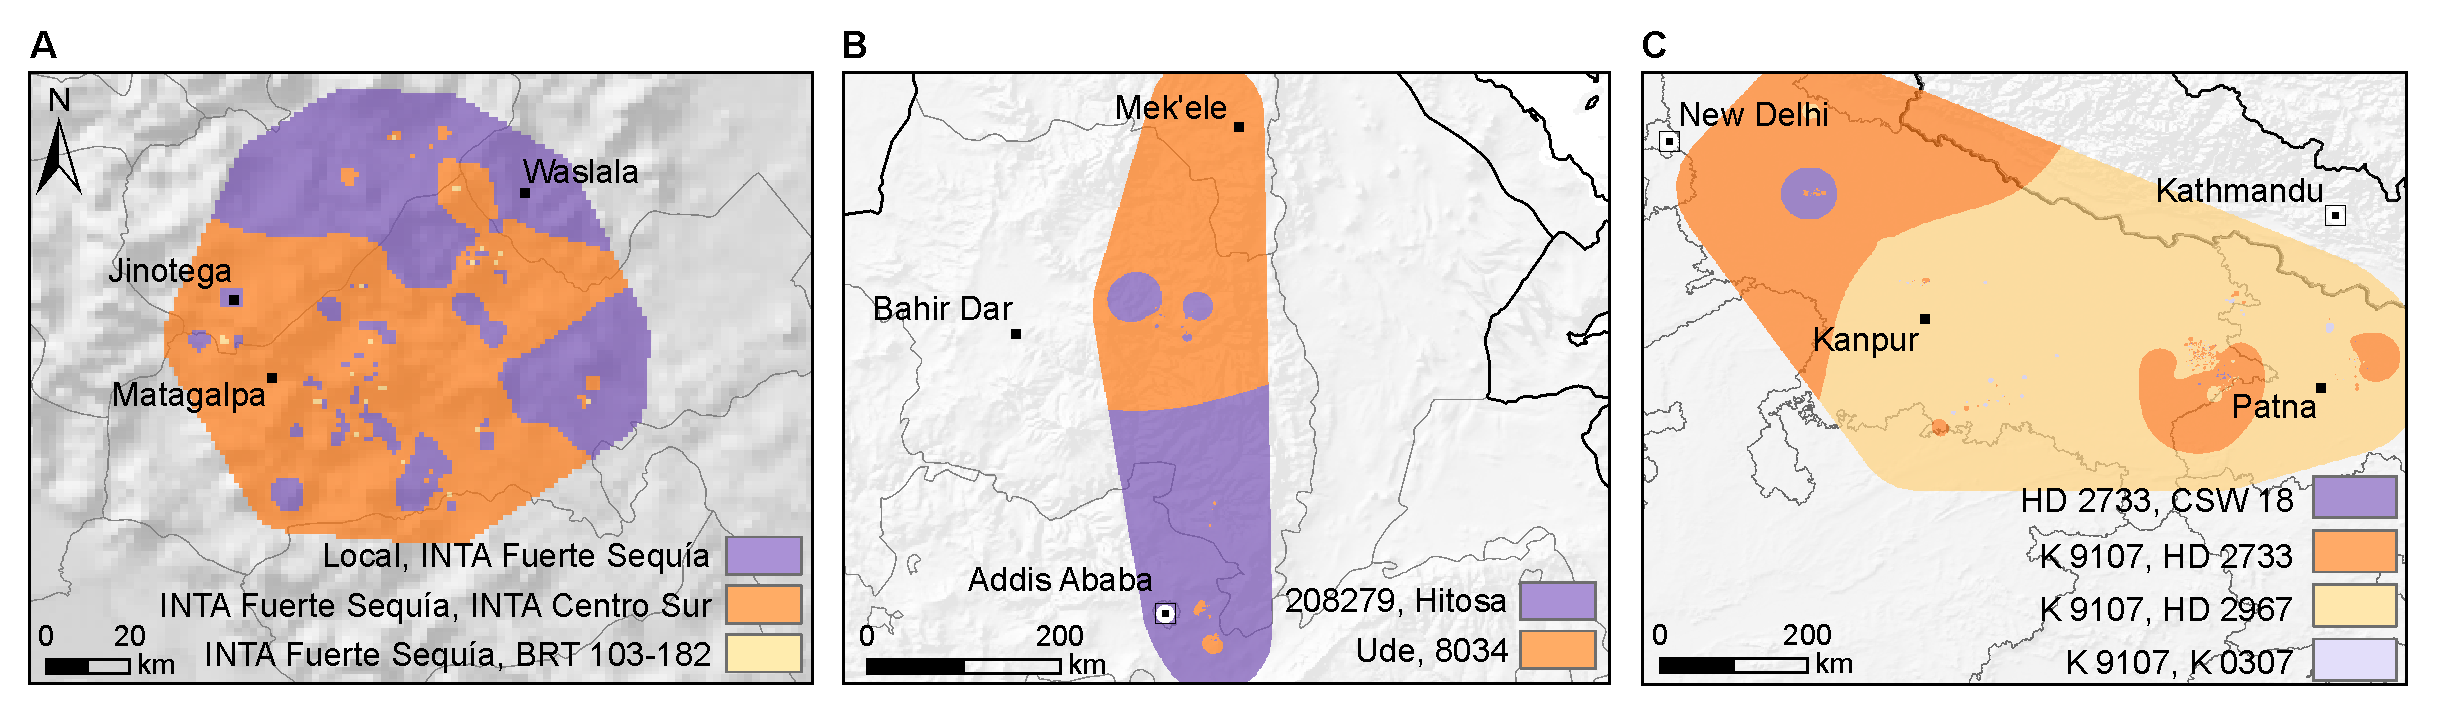
\includegraphics[width=1\textwidth]{Fig3_Recommendations.eps}
\caption{Variety recommendations based on average season predictions from Plackett-Luce trees using climatic variables for: \textit{(A)} common bean in Nicaragua (Apante season), \textit{(B)}  durum wheat in Ethiopia (Meher season), and \textit{(C)} bread wheat in India (Rabi season). Map categories show the top two varieties for each area according to their probability of winning over a base period (2002-2016).}
\label{fig:recommendations}
\end{figure*}

For Ethiopia, CIMMYT's \textit{Wheat Atlas} recommends modern varieties Hitosa, Ude, and Assassa for all of the Ethiopian highlands, which it classifies as a single ‘‘mega-environment’’ \cite{cimmyt2018atlas}. The tricot approach produced geographically more specific recommendations (Fig. 3\textit{B}). With this, we confirm the results of a previous analysis based on multi-locational trial data that showed the benefits of location-specific recommendation domains for durum wheat in Algeria, and we show that such an analysis can also be done with tricot data \cite{annicchiarico2006repeatable}. The tricot results confirmed the superiority of farmer varieties 8208 and 208304 (Table 3), which were approved for official variety release in March 2017 (on the basis of other field trials) \cite{mengistu2018genetic}. Farmer variety 208279 also has a high probability of winning, but has a high value of worst regret (Table 3). Our analysis suggests that 208279 could be considered for the coldest areas, as shown in Fig. 3\textit{B}. In Ethiopia, the tricot trial findings improve variety recommendations for durum wheat by uncovering the importance of cold adaptation.


For India, we compare our findings with the front-line demonstrations of the Indian Institute for Wheat and Barley Research (IIWBR), which are one-hectare plots that demonstrate new varieties by comparing them with a check variety. IIWBR promoted the variety HD 2967 for the North-Eastern Plain Zone during 2016-2017 \cite{icar2017progress}. HD 2967 was indeed the top variety in the tricot trial among the varieties considered by IIWBR (Table 3). In the tricot trials, however, K 9107 (a variety released in 1996) outperformed HD 2967 (released in 2011) with a comparable level of worst regret (Table 3). The tricot trials also showed that another variety, HD 2733, outperformed HD 2967 in a large part of the study area (Table 3). In the IIWBR front-line demonstrations, HD 2733 was included as a check variety in four areas and was outyielded by HD 2967 in only one of the four areas, while in the other three the yield difference was not significant \cite{icar2017progress}. Our analysis shows that HD 2733 generally does better than HD 2967 in areas with a low average diurnal temperature range during the growing season (Fig. 3\textit{C}). In India, the analysis of the tricot trial data adds geographic specificity to the existing variety recommendations, and suggests a broader set of wheat varieties should be promoted to take into account the climatic differences across the study area.

We quantified how much farmers can benefit from tricot-based variety recommendations by calculating variety reliability, the probability of outperforming a check variety (Methods -- equation [2]). For each location, we compared the tricot-recommended variety (Fig. 3) with the best-performing variety from the previous recommendations as the check. In Ethiopia, reliabilities range 0.59-0.65, in Nicaragua 0.58-0.60, and in India 0.51-0.62 (SI Appendix, Fig. S4), indicating substantial benefits for large areas.

\section*{Conclusions} 

The main question that we addressed is whether on-farm participatory crop trials, scaled through a farmer citizen science approach, can generate insights into climate adaptation of varieties. Citizen science data revealed generalizable relations between seasonal climate variables and crop variety performance that corresponded to known yield-determining factors. Climatic analysis of this data was shown to improve variety recommendations.
The novelty of our study is the demonstration that in vulnerable, low-income areas climatic analysis of variety performance is possible with trial data generated directly by farmer citizen scientists on farms. Arguably, similar results could be achieved by a combination of existing approaches (target environment characterization, multi-location trials, participatory variety selection, variety dissemination). The unique contribution of the tricot approach is that it integrates aspects of these approaches into a simple trial format that addresses the challenge of variety replacement for climate adaptation in a way that is at the same time scalable and demand-led. Tricot trials can track climate trends as they manifest themselves on farms, adjust variety recommendations and recommendation domains, and contribute to understanding how climate affects on-farm varietal performance. Trial analysis combines insights in climatic adaptation mechanisms with a comprehensive evaluation of variety performance from the perspective of farmers, the end-users of the seeds. Results can therefore be directly translated into actionable information for climate adaptation on the ground. The findings can serve to create variety portfolios that diminish climate risk \cite{sukcharoen2016mean}, can feed into climate information services in combination with seasonal forecasts \cite{klemm2017development}, and can become part of decentralized plant breeding strategies for climate adaptation \cite{ceccarelli2015efficiency}. Combining the tricot trial data with other data could generate additional insights into variety performance and acceptability as influenced by environmental \cite{minet2017crowdsourcing}, socio-economic \cite{hammond2017rural}, and genomic \cite{kidane2017genome} factors. 

The tricot approach facilitates engaging large numbers of farmers in citizen science trials with large sets of varieties. Scaling does not only involve an expansion in terms of numbers and scope, however, but also implies new institutional arrangements. Carefully designed strategies should foster communication between providers and users of information \cite{hewitt2017improving}. Wide-ranging collaborations are needed for climate adaptation in crop variety management, involving farmers, extension agents, seed retailers, seed producers, plant breeders, and climate information providers. The tricot approach can help to cut across these different domains, because it is able to link climatic and varietal information directly to farmer decision-making. With appropriate institutional support and investment, citizen science can potentially make an important contribution to farmers' adaptive capacity and to the mobilization of crop genetic diversity for climate adaptation.

\matmethods{
\subsection*{Crop trials}
Trials were performed between 2012 and 2016 during three cropping seasons in Ethiopia, five cropping seasons in Nicaragua, and four cropping seasons in India (SI Appendix, Table S1). Trial design followed the tricot citizen science approach \cite{van2016first,van2011crowdsourcing}. Sets of varieties were allocated randomly to farms as incomplete blocks \cite{atlin2001comparison}, maintaining spatial balance by assigning roughly equal frequencies of the varieties to each area. In Nicaragua and India, incomplete blocks contained three varieties. In Ethiopia, we used a modified approach that included four varieties per farm. Plots were small to facilitate farmer participation, but in all cases large enough to avoid strong edge effects. Farmers indicated the relative performance of varieties through ranking. Ranking is a robust data collection approach that avoids observer drift \cite{halekoh2008evaluation} and allows for aggregation across disparate datasets \cite{simko2011combining}. 

The trials required three moments of contact with the farmers: (1) explaining the experiment and distributing the seeds, (2) collecting evaluation data and (3) returning the results. Data were initially collected using paper forms and in subsequent seasons through electronic formats, linked to a purpose-built digital platform, ClimMob.net. In the trials presented here, field agents collected the data through visits (phone calls are also feasible).

\subsection*{Data analysis}
All analyses were done in R \cite{core2017R}. For the analysis of the variety ranking data generated by farmers, we used the Plackett-Luce model \cite{plackett1975analysis, luce1959individual}. The Plackett-Luce model estimates for each variety the probability that it wins, beating all other varieties in the set. The model determines the values of positive-valued parameters $\alpha_{i}$ (worth) associated with each variety $i$. These parameters $\alpha$ are related to the probability that variety $i$ wins against all other $n$ varieties in the following way.

\begin{equation} \begin{aligned}P ( i \succ \{ j , \cdots, n \} ) = \frac { \alpha _ { i } } { \alpha _ { 1 } + \cdots + \alpha _ { n } }\end{aligned} \end{equation}
The probability that variety $i$ beats another variety $j$ is calculated in a similar way.
\begin{equation} P ( i \succ j ) = \frac { \alpha _ { i } } {\alpha _ { i } + \alpha _ { j } }\end{equation}
Equation [2] also serves to calculate the reliability of a variety -- its probability of beating a check variety \cite{eskridge1992choosing}. These equations follow from Luce’s Choice Axiom, which states that the probability that one item beats another is independent from the presence or absence of any other items in the set \cite{luce1959individual}. We report worth values that sum to 1. This makes each worth value $\alpha_i$ equal to the probability of variety $i$ outperforming all other varieties. 
\begin{equation} P ( i \succ \{ j , \cdots, n \} ) = \frac { \alpha _ { i } } { \alpha _ { 1 } + \cdots + \alpha _ { n } } = \frac { \alpha _ { i } } { 1 } = \alpha _ { i }\end{equation}
In the trials, we used rankings of three varieties ($i \succ j \succ k$), which have the following probability of occurring according to the Plackett-Luce model.
\begin{equation} P ( i \succ j \succ k ) = P ( i \succ \{ j , k \} ) \cdot P ( j \succ k ) \end{equation}
The log-likelihood for a ranking $i \succ j \succ k$ follows from equations [1], [2] and [4] and takes the following form \cite{hunter2004mm}.
\begin{equation} \begin{aligned} \ell ( \boldsymbol { \alpha } ) & = \ln ( P ( i \succ \{ j , k \} ) ) + \ln ( P ( j \succ k ) ) \\ & = \ln \left( \alpha _ { i } \right) - \ln \left( \alpha _ { i } + \alpha _ { j } + \alpha _ { k } \right) + \ln \left( \alpha _ { j } \right) - \ln \left( \alpha _ { j } + \alpha _ { k } \right) \end{aligned} \end{equation}
The log-likelihood is then the sum of the log-likelihood $\ell ( \boldsymbol { \alpha } )$ values across all rankings. Using an iterative algorithm, the log-likelihood is maximized to identify the $\alpha$ values that make the observed rankings most probable. We also generated quasi standard errors for $\alpha$ \cite{turner2018modelling}. To take into account covariates, we created Plackett-Luce Trees (PLT) through recursive partitioning \cite{strobl2011accounting}. Further details are given in the SI Appendix.

\subsection*{Data and code availability} Full data is available through Dataverse \cite{vanettenreplic}. Code is available as SI Appendix, Code S1.

\subsection*{ACKNOWLEDGEMENTS}
We thank all farmers who evaluated varieties in Nicaragua, Ethiopia and India. Part of this research was supported by cooperative agreement AID-OAA-F-14-00035, which was made possible by the generous support of the American people through the United States Agency for International Development (USAID). The research received financial support from McKnight Foundation (CCRP 16-098), the German Federal Ministry for Economic Cooperation and Development (BMZ/GIZ, Contract No. 81194988) and the Indian Council of Agricultural Research (ICAR, Annual Workplan). This work was implemented as part of the CGIAR Research Program on Climate Change, Agriculture and Food Security (CCAFS), which is carried out with support from the CGIAR Trust Fund and through bilateral funding agreements. For details please visit https://ccafs.cgiar.org/donors. The views expressed in this document cannot be taken to reflect the official opinions of these organizations. We thank Vincent Johnson and Olga Spellman for editorial support and Heather Turner for support on scientific programming.
}
\showmatmethods{}
\pnasbreak
% \pnasbreak splits and balances the columns before the references.
% Uncomment \pnasbreak to view the references in the PNAS-style
% If you see unexpected formatting errors, try commenting out \pnasbreak
% as it can run into problems with floats and footnotes on the final page.
%\pnasbreak

% Bibliography
\bibliography{pnas-sample}

\end{document}